\chapter{Polarization of single top quarks in \textsl{t}~channel at 8~TeV}

\intro{A first measurement of the top quark spin asymmetry in t~channel, related to the top quark polarization, is presented in this chapter. Proton-proton collision data at $\mathit{\sqrt{s}=8}$~TeV have been analyzed corresponding to about $\mathit{20~fb^{-1}}$. Events with an isolated muon are selected together with two or three jets for the final measurement while events containing an isolated electron and jets have been studied as well. The normalized differential cross section is measured as a function of the polarization angle. From its shape, a spin asymmetry of $\mathit{0.26\pm0.03~(stat)\pm0.10~(syst)}$ is obtained. This is found to be compatible within $\mathit{2.0}$ standard deviations with the expected \gls{sm} asymmetry of $\mathit{0.44}$. The result has been published in Ref.~\cite{Khachatryan:2015dzz}. In a further step, the derivation of limits on anomalous couplings is illustrated by combining this measurement with related ones.}

The strategy to measure the top quark spin asymmetry is as follows. After event selection, two \glspl{bdt} are trained. The first one is optimized to reject events with fake leptons stemming from multijet production. The second \gls{bdt} is then trained to separate signal from \wjets and \ttbar events. 





\section{Simulated samples and event selection}

separating, W+HF, W+LF
categorization (2j0t,2j1t,...)
QCD estimation

\myfigure{\label{fig:polarization-categorization}Categorization of events depending on number of selected jets, number of b-tags, and the signal \gls{bdt} discriminant.}{
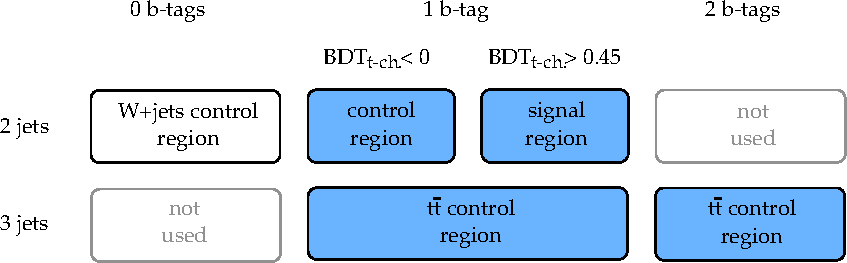
\includegraphics[scale=0.75]{figures/polarization/regions.pdf}
}

all plots scaled to fit result unless stated otherwise


\section{Training of Boosted Decision Trees}


\myfigure{\label{fig:polarization-qcdbdt-inputs}Distributions of \gls{bdt} input observables, (a)~missing transverse energy, (b)~top quark mass, (c)~transverse W~boson mass, (d)~untagged jet $\pt$, (e)~isotropy; and (f)~the distribution of the final \gls{bdt} discriminant for rejecting multijet events.}{
\subfloat[]{\adjincludegraphics[height=4.8cm,trim={0 0 {0.23\width} 0},clip]{figures/polarization/2j1t/muon_2j1t_met_qcdnone_nol.pdf}}
\hspace{0.017\textwidth}
\subfloat[]{\adjincludegraphics[height=4.8cm]{figures/polarization/2j1t/muon_2j1t_top_mass_qcdnone.pdf}}\\
\subfloat[]{\adjincludegraphics[height=4.8cm,trim={0 0 {0.23\width} 0},clip]{figures/polarization/2j1t/muon_2j1t_mtw_qcdnone_nol.pdf}}
\hspace{0.017\textwidth}
\subfloat[]{\adjincludegraphics[height=4.8cm]{figures/polarization/2j1t/muon_2j1t_ljet_pt_qcdnone.pdf}}\\
\subfloat[]{\adjincludegraphics[height=4.8cm,trim={0 0 {0.23\width} 0},clip]{figures/polarization/2j1t/muon_2j1t_isotropy_qcdnone_nol.pdf}}
\hspace{0.017\textwidth}
\subfloat[]{\adjincludegraphics[height=4.8cm]{figures/polarization/2j1t/muon_2j1t_bdt_qcd_qcdnone.pdf}}
}

\myfigure{\label{fig:polarization-signalbdt-inputs}Distributions of input observables used in the training of the \gls{bdt} discriminant for separating signal from \wjets and \ttbar events.}{
\subfloat[]{\adjincludegraphics[height=4.8cm,trim={0 0 {0.23\width} 0},clip]{figures/polarization/2j1t/muon_2j1t_ljet_abseta_qcdbdt_nol.pdf}}
\hspace{0.017\textwidth}
\subfloat[]{\adjincludegraphics[height=4.8cm]{figures/polarization/2j1t/muon_2j1t_bjet_abseta_qcdbdt.pdf}}\\
\subfloat[]{\adjincludegraphics[height=4.8cm,trim={0 0 {0.23\width} 0},clip]{figures/polarization/2j1t/muon_2j1t_bjet_mass_qcdbdt_nol.pdf}}
\hspace{0.017\textwidth}
\subfloat[]{\adjincludegraphics[height=4.8cm]{figures/polarization/2j1t/muon_2j1t_bjet_pt_qcdbdt.pdf}}\\
\subfloat[]{\adjincludegraphics[height=4.8cm,trim={0 0 {0.23\width} 0},clip]{figures/polarization/2j1t/muon_2j1t_shat_logmass_qcdbdt_nol.pdf}}
\hspace{0.017\textwidth}
\subfloat[]{\adjincludegraphics[height=4.8cm]{figures/polarization/2j1t/muon_2j1t_hfs_logpt_qcdbdt.pdf}}
}

%choice of variables, correlation tests

\section{Signal extraction}

\section{W+jet modeling}

\section{Validation}

cosTheta, cosWhel, top mass in SR/CR, 2j0t,3j1t

\section{Unfolding}

bdt cut, neyman construction

\section{Statistical evaluation}

Q-scale reweighting, chi2 fit

\section{Results}

\myfigure{}{
\subfloat[]{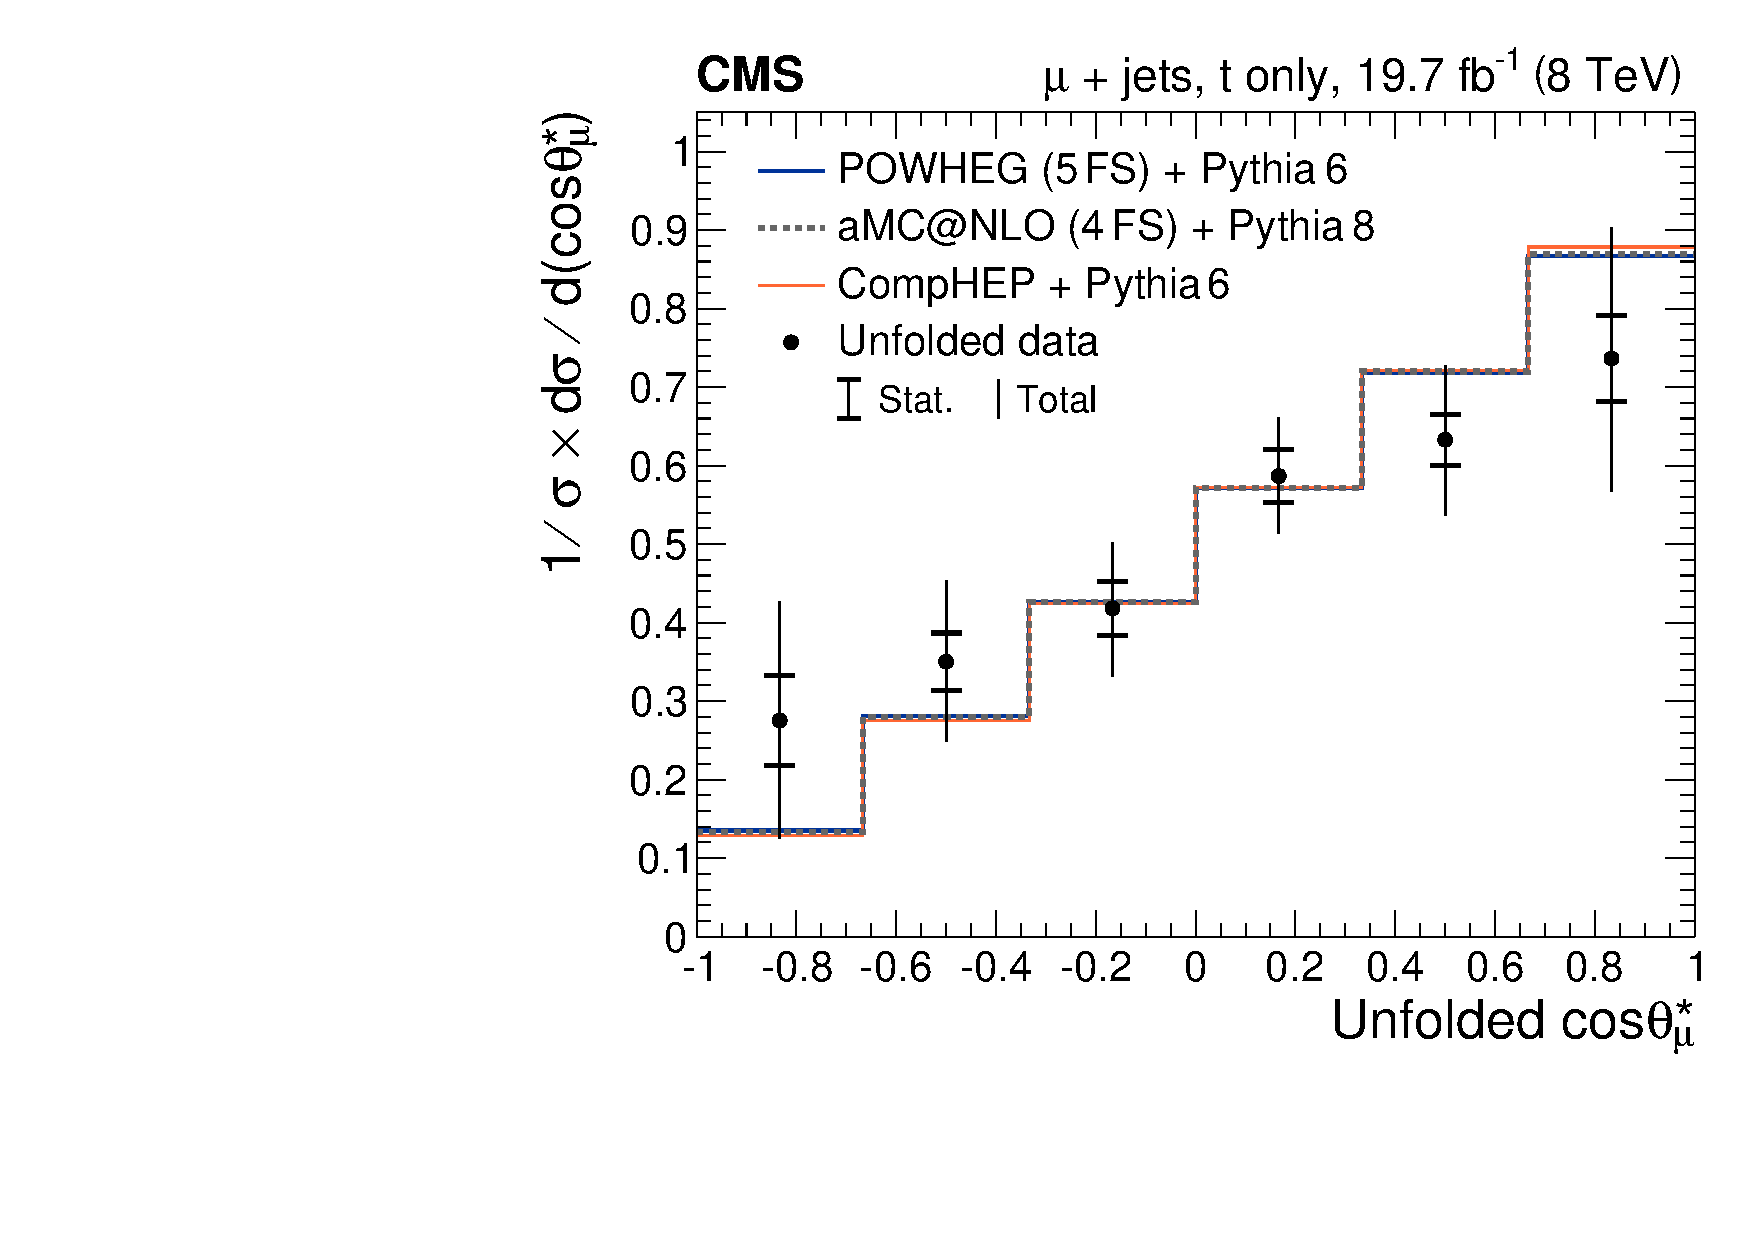
\includegraphics[width=0.48\textwidth]{figures/polarization/result/unfolded_mu_top.pdf}}
\hspace{0.02\textwidth}
\subfloat[]{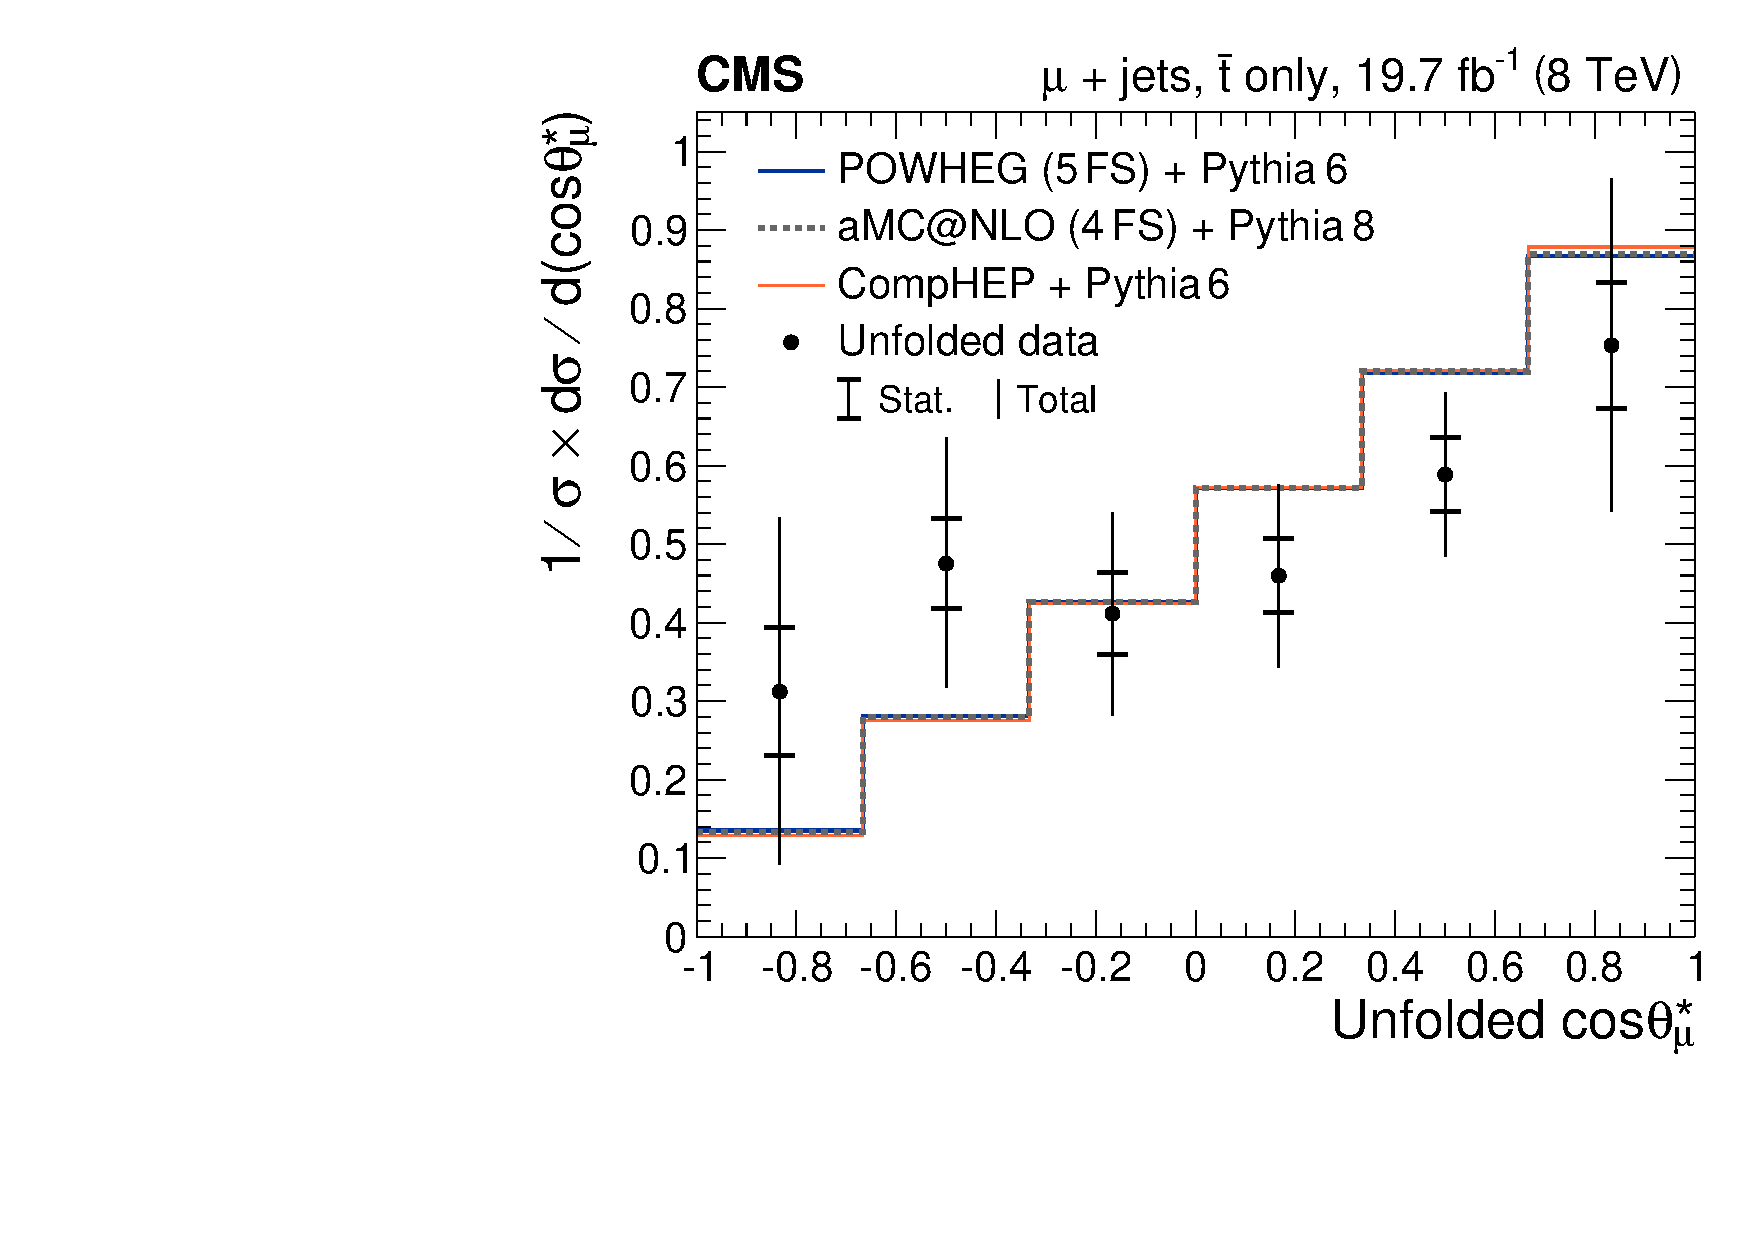
\includegraphics[width=0.48\textwidth]{figures/polarization/result/unfolded_mu_antitop.pdf}}\\
\subfloat[]{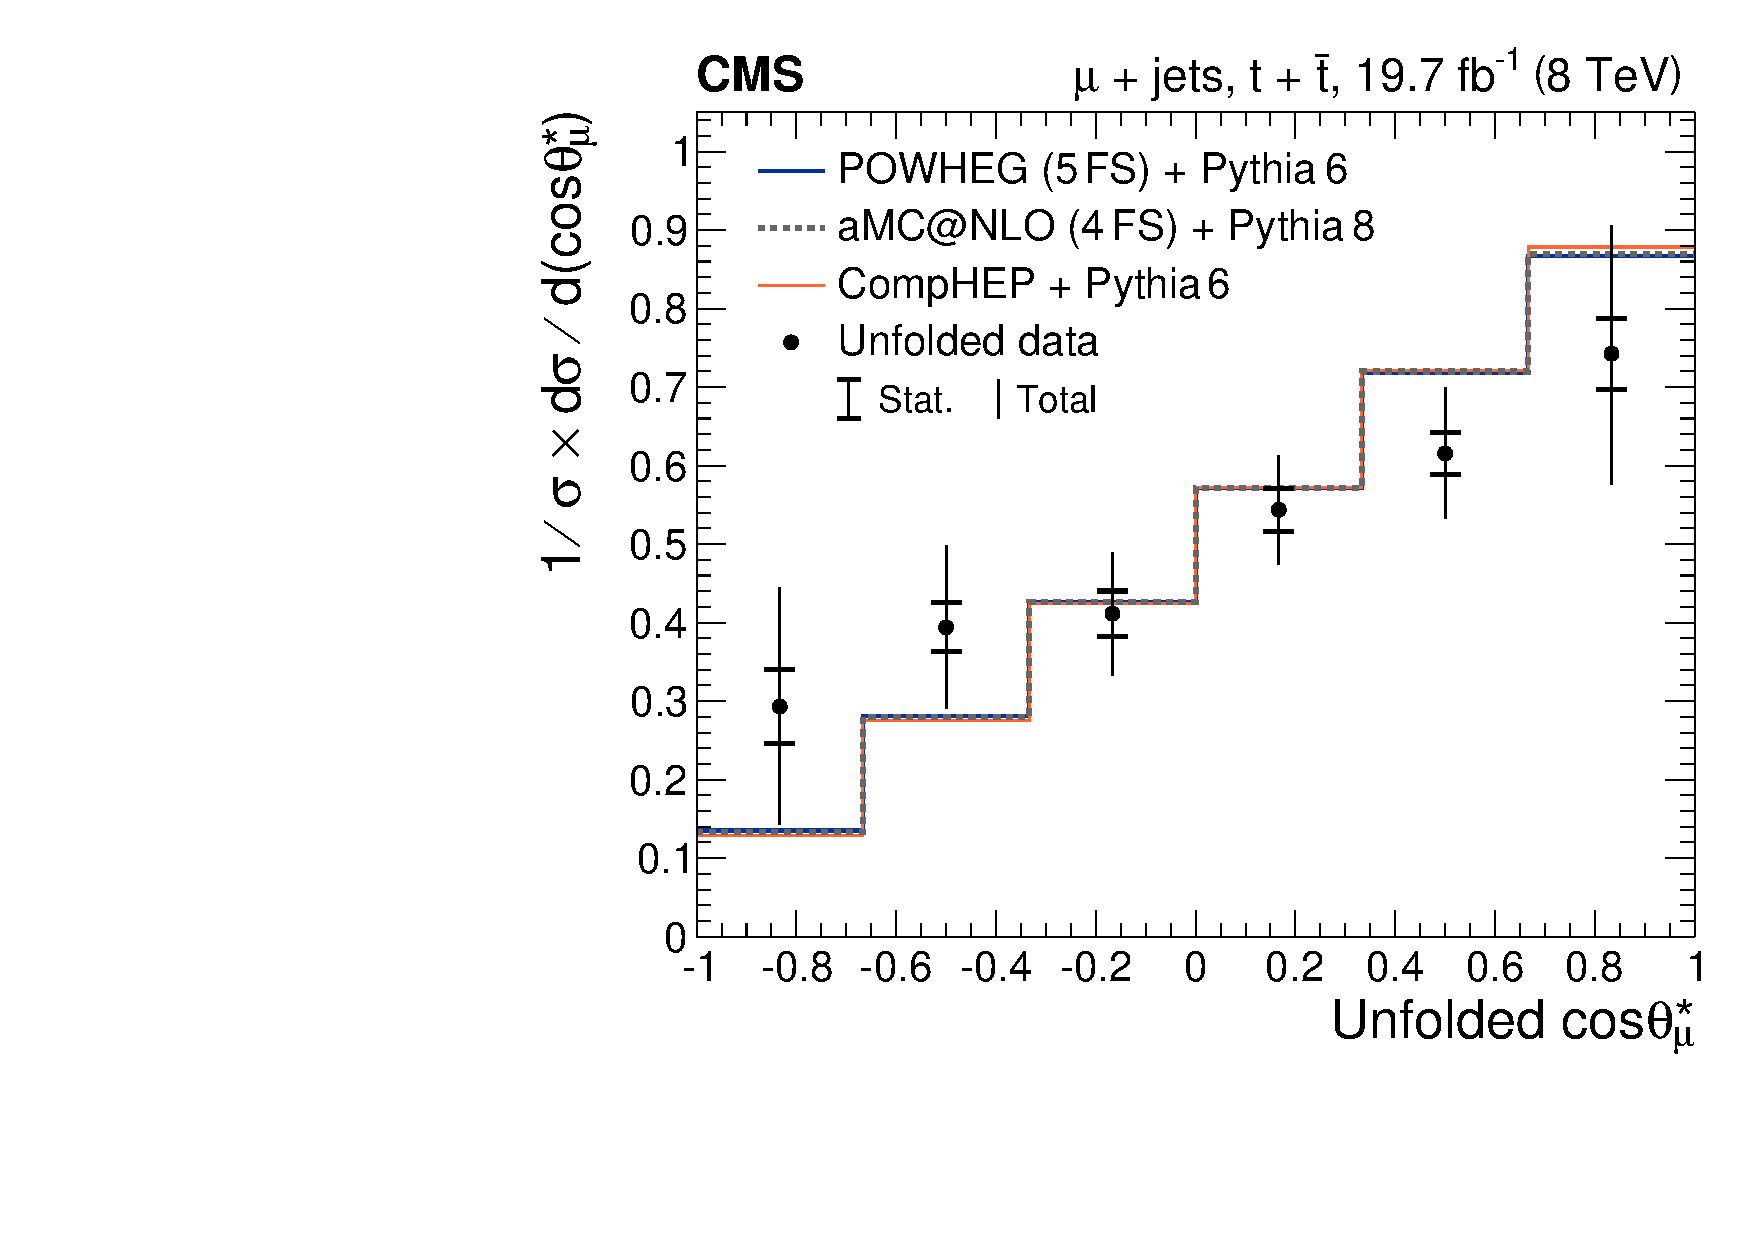
\includegraphics[width=0.48\textwidth]{figures/polarization/result/unfolded_mu.pdf}}
}

\section{Limits on anomalous couplings}

topfit